\documentclass[12pt, a4paper, notitlepage, twocolumn]{article}

\usepackage{graphicx}
\usepackage{authblk}
\usepackage[left=1.5cm, right=1.5cm, top=2cm, bottom=2cm]{geometry}
\usepackage{hyperref}
\usepackage{amsmath}

\graphicspath{{images/}}

\title{\textbf{Augmented Sentinel 1-2 Dataset for SAR optical translation}}

\author[1]{Shamba Chowdhury}
\author[1]{Ankana Ghosh}
\author[1]{Shreyashi Ghosh}

\affil[1]{\small{Department of Computer Science and Engineering, University of Calcutta}}

\date{April 2025}

\begin{document}

\twocolumn[
    \begin{@twocolumnfalse}
        \maketitle

        \begin{abstract}
            Deep learning techniques are having a major impact on every technical fields now-a-days and gathering sufficient amounts of training data was challenging in the space of remote sensing. This problem was solved by the Sen 1-2 dataset\cite{tumsen12}. The dataset contains almost 300,000 pairs of SAR and optical images across multiple seasons and regions. We have extended the dataset with an additional XX pair of images. Furthermore, the dataset has been augmented with temperature region information for all images. We believe that this data augmentation will help in the progression of various SAR image applications.
        \end{abstract}
    \end{@twocolumnfalse}
]

\section{Introduction}
The TUM Sentinel 1-2 dataset is widely used in various remote sensing computer vision tasks. It consists of 282,384 pairs of SAR and optical images. This massive amount of data has enabled various applications of deep generative networks in the field of remote sensing\cite{Zhang2023}.

In this extension of the dataset, we have augmented it with an addition of XX pairs of SAR and optical images, increasing the diversity and coverage. Furthermore, we have introduced a novel temperature region annotation for each image, providing valuable metadata that we believe will enable better research workflow. This augmented dataset facilitates more precise and context-aware deep learning models for tasks such as SAR to optical image translation.

This paper provides an overview of the dataset extension, its structure, the methodology of acquiring the data, and some use cases.

\section{The SEN1-2 Dataset}
The SEN1-2 dataset contains 282,384 pairs of SAR and optical image patches extracted from versatile Sentinel-1 and Sentinel-2 scenes. These are $256\times256$ RGB images in png format. The images (or patch pairs) were selected by randomly selecting various regions (called scenes) and then segregated into four different seasons. The following table states the structure of the dataset in numbers:

\begin{table}[h!]
    \begin{center}
        \begin{tabular}{|c|c|c|c|}
            \hline
            Seed & Season & Scenes & Pairs \\
            \hline
            1158 & Spring & 70 & 75,724 \\
            1868 & Summer & 49 & 53,508 \\
            1970 & Fall & 78 & 86,370 \\
            2017 & Winter & 61 & 66,782 \\
            \hline
        \end{tabular}
    \end{center}
    \caption{Structure of the SEN1-2 Dataset}
    \label{table:senStruct}
\end{table}

The following points explain the significance of each column:
\begin{itemize}
    \item \textbf{Seed:} The number used to seed the RNG for the selection of the region.
    \item \textbf{Season:} The time period from the time the image is taken.
    \item \textbf{Scenes:} The total number of regions chosen globally.
    \item \textbf{Pairs:} The total number of patch-pairs or pairs of images from all the regions for that particular season.
\end{itemize}

\section{The Dataset}
The dataset format remains unchanged. The pairs of images are divided between 4 seasons and are grouped by regions into specific folders. However, the data acquisition process has been slightly changed. In addition to using Google Earth Engine\cite{GORELICK201718} we also use the Copernicus Data Space Ecosystem API to access Sentinel data.

\subsection{Image format}
The images are in png format with a dimension of $256\times256$ pixels. The scale or zoom level of the image in terms of distance is 20m. Now, the sentinel satellite-specific image details will be defined in the following points:
\begin{itemize}
    \item \textbf{Sentinel-1:} The images are taken from the IW acquisition mode of the satellite and are in VV polarization. It comprises of only a single band.
    \item \textbf{Sentinel-2:} The images consist of 3 bands for Red, Green, and Blue. The bands are also scaled for proper visualization.
\end{itemize}

\subsection{Heat Zone CSVs}
Each region folder in each season folder in the dataset comes with an accompanying csv file called \texttt{info\_XX}. The columns in the CSV are 's1\_fileName', 's2\_fileName', 'season' and 'region'. These CSV files contain the temperature region or the heat zone information for every image in the dataset.

\subsection{Copernicus API Method}
Copernicus Data Space Ecosystem with a tagline of Europe's eyes on Earth is an open ecosystem that provides free instant access to a wide range of data and services from the Copernicus Sentinel missions\cite{copernicusHome}. It provides data from all Sentinel satellites in various forms. For Sentinel-1 images, we used the 'Level 3 Monthly Mosaics' collection, and for Sentinel-2 we used the 'Level 3 Quaterly Mosaics' collection.
The following sections contain an overview of how the copernicus API was used to obtain the images.

\subsubsection{Generating coordinates}
The Copernicus service provides a limited number of API calls per month for free users (30,000 calls). To maximize efficiency of API call usage, we decided to obtain images of the maximum size limit offered by Copernicus. The maximum limit is $2500\times2500$ pixels per image. Now, the scale of images in SEN1-2 dataset is 20m.

\begin{align*}
    \text{Hence, ground distance per pixels} &= 20m \\
    \text{Total distance for 2500x image is} &= 20\times2500 \\
    &= 50,000m
\end{align*}

Thus, we need to create square patches with 50 KM distances as the side of the said patch. For this task, we first select a region in Google Earth Engine using the rectangular selection tool. We can then obtain the coordinates for the four corners of the selection. We use these coordinates to divide the region into multiple square regions with 50 KM side. To perform the division, we calculate the subsequent latitude and longitude coordinates beginning from the top left corner of the selection. The formulas for approximately converting longitude and latitude into kilometers are as follows:

\begin{itemize}
    \item \textbf{Latitude: } $1^\circ = 110.574$KM
    \item \textbf{Longitude:} $1^\circ = 111.320\times cos(latitude)$ KM
\end{itemize}

Thus, we end up with a list of coordinates for all subregions formed from the original selection.

\subsubsection{Authentication} \label{CopeAuth}
In order to use the API of copernicus sentinel hub, we need to authenticate ourselves and obtain an access token. Therefore, client id and client secret are used to fetch a token and authenticate ourself.

\subsubsection{Defining Image properties} \label{CopImgProp}
AFter authentication, the image properties are set in preparation of the image download. This is where the difference in obtaining Sentinel-1 and Sentinel-2 images appear due to differences in image formats.

We set the image height and width to 2500 pixels each. Following that, the eval script is set. An eval script is a piece of Javascript code which defines how the satellite data shall be processed by Sentinel Hub\cite{evalDoc}. Two different eval scripts are used for Sentinel-1 and Sentinel-2 images due to the different number of bands being used in the images.

The Sentinel-1 eval script is as follows:

\begin{lstlisting}
    //VERSION=3
    function setup() {
        return {
            input: ["VV"],
            output: { bands: 1 }
        };
    }

    function evaluatePixel(sample) {
        return [sample.VV];
    }
\end{lstlisting}

The Sentinel-2 eval script is as follows:

\begin{lstlisting}
    //VERSION=3
    function setup() {
        return {
            input: ["B02", "B03", "B04"],
            output: { bands: 3 }
        };
    }

    function evaluatePixel(sample) {
        return [2.5 * sample.B04/10000, 2.5 * sample.B03/10000, 2.5 * sample.B02/10000];
    }
\end{lstlisting}

From the eval scripts we can infer that Sentinel-1 images have one band, called "VV". It is the polarization of the captured image. "VV" is vertical polarization, i.e.,  vertically transmit and vertically receive. And Sentinel-2 images have 3 bands, namely, B02, B03, B04. The bands are for Blue, Green, and Red channel respectively. The Sentinel-2 images are also preprocessed before download by scaling and normalizing the pixel values. 

Then, bounding box coordinates and time frame for images are sent with the request along with the previously mentioned data.

\subsubsection{Adding Region Data}
Now, the new addition to our dataset is the temperature region information. Temperature regions are also known as heat zones of the Earth. There are three heat zones, Arctic or Frigid zone, Temperate zone, and Tropical or Torrid Zone. These zones are classified according to latitude.

\begin{itemize}
    \item Tropical Zone: It lies between the Tropic of Cancer ($23.5^\circ$ North) and Tropic of Capricorn ($23.5^\circ$ South). This zone receives the most heat from the sun.
    \item Temperate Zone: In the northern hemisphere, this zone lies between Tropic of Cancer and the Arctic circle ($66.5^\circ$ North). In the southern hemisphere, it lies between Tropic of Capricorn and Antarctic circle ($66.5^\circ$ South).This region is moderately cooler compared to the tropical region.
    \item Arctic Zone: In the northern hemisphere, it is located between the North Pole ($90^\circ$ North) and Arctic circle. In the southern hemisphere, it lies between the South Pole ($90^\circ$ South) and the Antarctic circle. This region is the coldest region of them all.
\end{itemize}

We have decided to include lesser amounts of arctic zone data, as those images are mainly composed of snow without much variation.

Therefore, the region is calculated based on the latitude and is written to a csv file. The csv files are made on a per region folder basis.

\subsubsection{First manual inspection}
Once the images are downloaded, the first manual inspection is performed. We check the pair of images to verify that the images contain visible patterns and variations throughout its entirety. Images which had regions of no variation were discarded.

Moreover, unlike the original dataset, cloud coverage was not an issue as the Sentinel-2 Monthly Mosaics were cloud optimized images.

\subsubsection{Cropping images}
After the first manual inspection, the images were cropped and divided into multiple smaller images to match the dimensions of the original dataset. The downloaded images have a dimension of $2500\times2500$ pixels. They are divided into 81 $256\times256$ sized images each. This results in a minor loss of information. Figure \ref{fig:cropStep} shows the visualisation of this step.

\begin{figure*}
    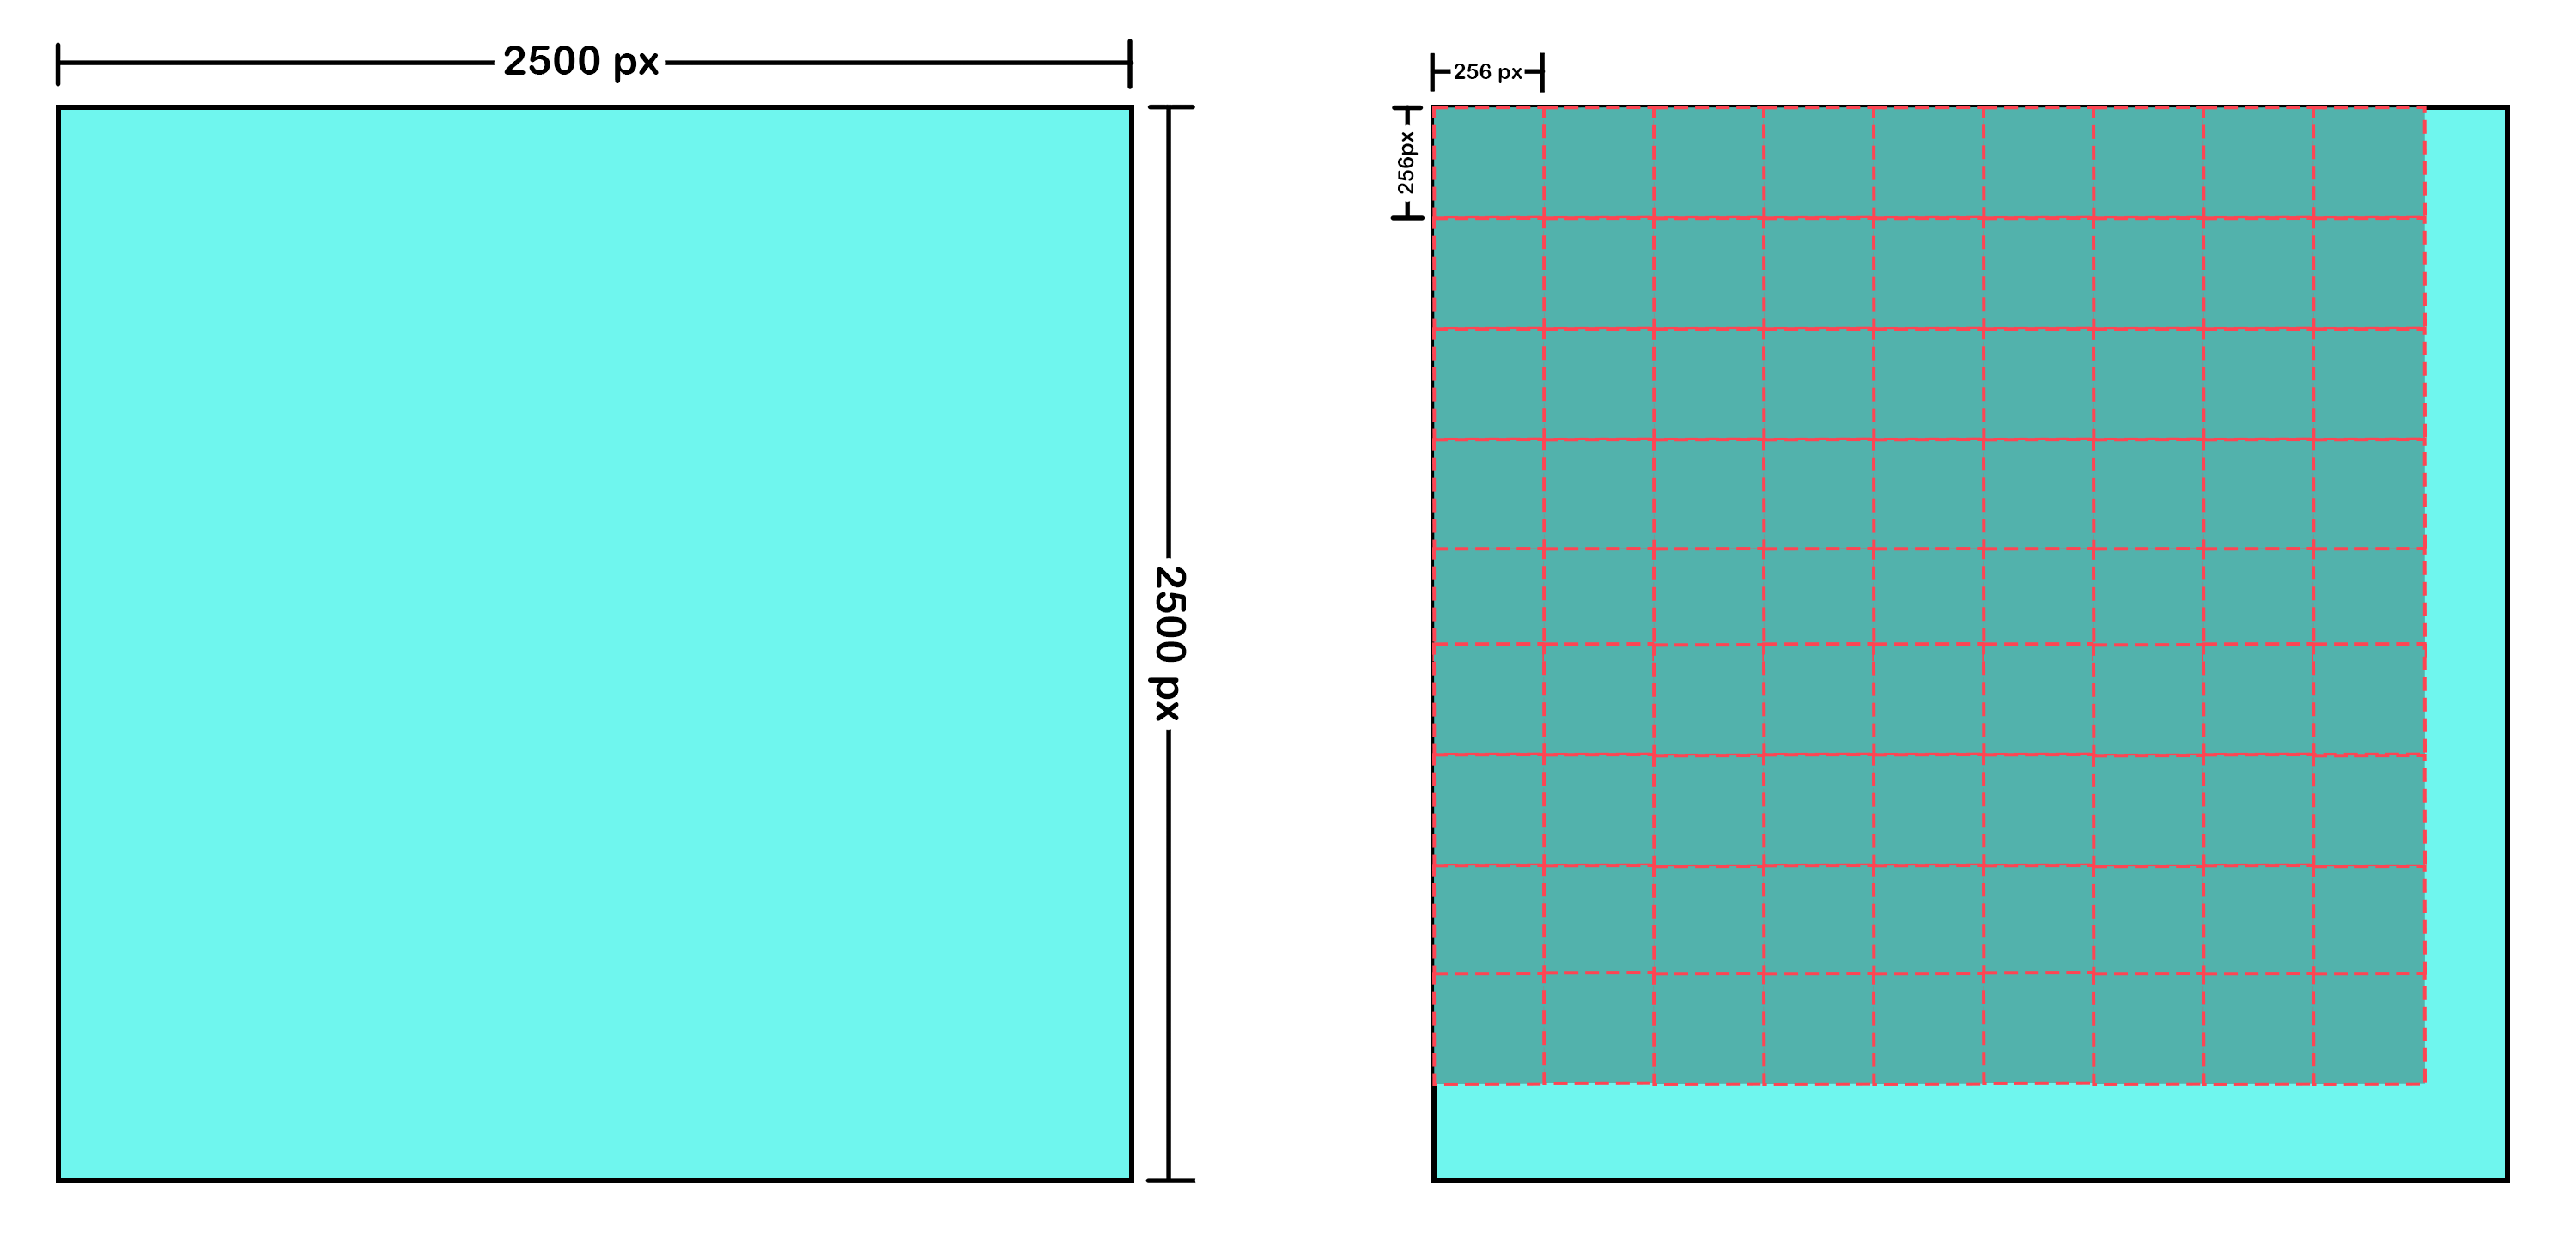
\includegraphics[width=\textwidth]{cropStep.png}
    \caption{Image demonstrating the step of cropping and dividing the large image into smaller images.}
    \label{fig:cropStep}
\end{figure*}

\begin{figure*}[t]
    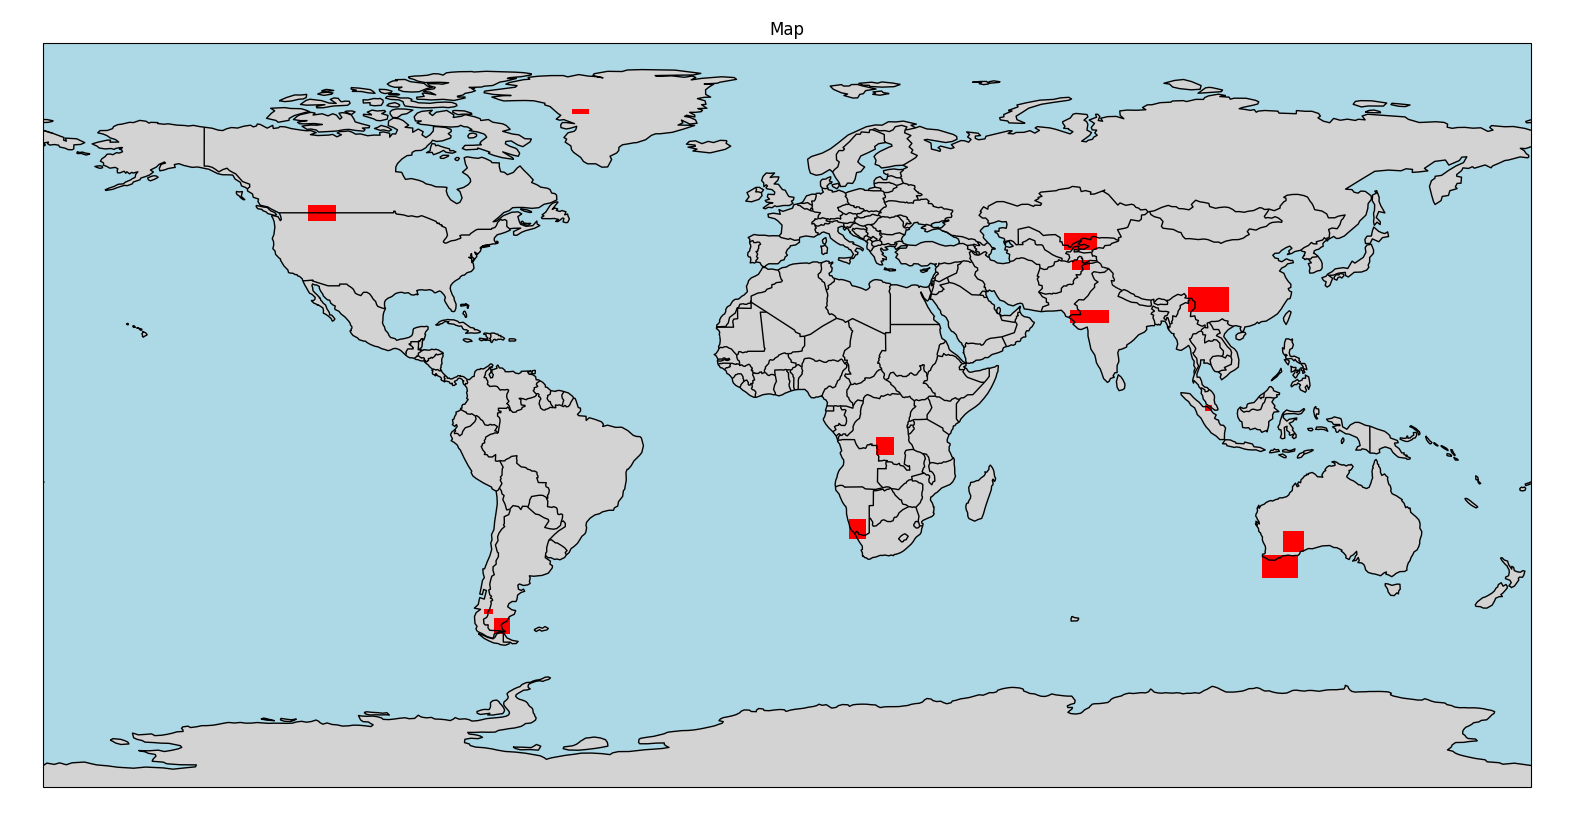
\includegraphics[width=\textwidth]{worldMap.png}
    \caption{Additional scenes (marked in red) for new set of patch pairs.}
    \label{fig:newMap}
\end{figure*}

\subsubsection{Second manual inspection}
Once the images are cropped and divided into smaller images, one last manual inspection is performed. The purpose of this inspection is the same as the first manual inspection, to verify variations in images. This check is performed to ensure no plain images exist in the dataset.

\subsection{Google Earth Engine Method}
The second method that we have used to extend the already existing datasets is using the \textbf{Google Earth Engine (GEE)}. Google Earth Engine is a cloud-based geospatial analysis platform that enables users to visualize and analyze satellite images of our planet. In this section, we have extended the Sentinel-1 and Sentinel-2 datasets by keeping the original dataset formats intact.

We have selected 8 regions on the world map and stored them as variables. Then we have defined the regions with their corresponding seasons, date ranges and folder names. We are considering 4 seasons - \textit{Spring, Summer, Fall} and \textit{Winter} with folder numbers - 149, 142, 146 and 147 respectively. Each season will contain data for both Sentinel-1 and Sentinel-2.

We have also distinguished the regions based on their temperature regions,i.e., - \textit{Tropical, Temperate and Arctic}.

For each region, we are randomly generating \textbf{500 sample points(sample point dimension : 256 * 256 pixels, zoom level : 20m)}. For each point, we are identifying its temperature zone, then generating their Sentinel-1 and Sentinel-2 mosaics and exporting them. For Sentinel-1 images, we are selecting images in \textbf{IW mode with VV polarization} and for Sentinel-2 images, we are selecting images with \textbf{bands B4, B3 and B2} (i.e., red, green and blue channels). The script is as follows:

Finally, we are creating a CSV file with the following columns:
\begin{itemize}
    \item Sentinel-1 image file path
    \item Sentinel-2 image file path
    \item Prompt(Season and Temperature Region Information)
    \item Sentinel-1 image
    \item Sentinel-2 image
\end{itemize}
And, exporting the CSV file to Google drive using the \textbf{\texttt{Export.table.toDrive}} function.


\subsection{Augmenting Dataset with Heat Zone}
In this enhancement of the dataset, we implement a new method that facilitates temperature zone labeling by identifying the best-matching Sentinel-2 images from the Copernicus API for each dataset image.

This method involves fetching high-resolution Sentinel-2 imagery for selected coordinates across different seasons, dividing them into smaller image patches, and comparing them with patches from the TUM Sentinel 1-2 dataset through feature-based image matching. This approach allows precise geographic tagging and classification of dataset images according to their hemisphere and temperature zone.

\subsubsection{Filtering ROI Coordinates}

We begin by extracting the relevant coordinate points from the \texttt{seasonal\_regions\_coordinates.csv} file, which is filtered based on the specific season under study (e.g., spring, summer, fall, or winter). Each row in the file includes a pair of latitude and longitude values representing a distinct geographical location.

This CSV was generated using the seasonal region map referenced in [1], where global areas are visually segmented by season through color-coded highlights. To automate the extraction process:

\begin{itemize}
    \item The map image was converted to the HSV color space using OpenCV.
    \item Color thresholds were defined to identify regions corresponding to each season:
    \begin{itemize}
        \item \textbf{Blue for winter} 
        \item \textbf{Red for fall}
        \item \textbf{Green for summer}
        \item \textbf{Orange for spring}
    \end{itemize}
    \item Contours were detected for each seasonal color, and the centroid of every contour was computed.
    \item Assuming an equirectangular map projection, the pixel-based centroids were converted into approximate latitude and longitude coordinates.
    \item These points were stored season-wise in the resulting CSV file.
\end{itemize}

\subsubsection{Retrieving Sentinel-2 Data via Copernicus API}

To obtain Sentinel-2 imagery, we make use of the Copernicus Data Space Ecosystem API. Authentication is handled securely using OAuth 2.0, where credentials in the form of a \texttt{client-id} and \texttt{client-secret} are used to establish an authorized session.

The procedure for defining image parameters, specifying the time range, and applying the \texttt{evalscript} to extract RGB bands (B02, B03, and B04) follows the methodology described earlier in Sections \ref{CopeAuth} and \ref{CopImgProp}.

For each coordinate, a high-resolution image of size 2500 × 2500 pixels is requested, centered around the specified location. This image forms the basis for subsequent segmentation and matching tasks.

\subsubsection{Segmenting the Images into 256×256 Image Patches}

Each $2500\times2500$ image is divided into 81 smaller patches, each sized 256 × 256 pixels. These patches are stored in season-specific folders and maintain compatibility with the original SEN1-2 dataset format.

\subsubsection{Feature Matching Using ORB}

For every \texttt{s2\_XX} folder in the dataset:

\begin{itemize}
    \item A random image is chosen as the target.
    \item ORB (Oriented FAST and Rotated BRIEF) feature descriptors are used to compare this image with each downloaded Sentinel-2 patch.
    \item A matching score is calculated based on the number of matched keypoints.
    \item The patch with the highest score is considered the best match.
\end{itemize}

\subsubsection{Classifying by Temperature Zone}

After identifying the best match, the latitude of the associated coordinate is used to determine its temperature zone:

\begin{itemize}
    \item \textbf{Tropical Zone:} Between -23.5° and +23.5°
    \item \textbf{Temperate Zone:} Between ±23.5° and ±66.5°
    \item \textbf{Arctic Zone:} Above ±66.5°
\end{itemize}

This classification is appended as metadata to each matched image.

\subsubsection{Output and Metadata Storage}

All results—including folder name, ORB match score, and temperature zone—are recorded in a season-specific CSV file. Each row provides:

\begin{itemize}
    \item The dataset folder name (\texttt{s2\_folder})
    \item The computed match score (\texttt{match\_score})
    \item The determined temperature zone (\texttt{temperature\_zone})
\end{itemize}

This structured CSV serves as an annotated index for geolocation and climatic zone metadata, enhancing the contextual utility of the dataset.

\subsubsection{Removed data}
A small portion of data was removed during this step as they couldn't be tagged properly with a matching region. The following regions from each season were removed: 

\begin{itemize}
    \item \textit{fall}: 4, 8, 13, 66, 82
    \item \textit{spring}: 45, 68, 95
    \item \textit{summer}: 53
    \item \textit{winter}: 12
\end{itemize}

In total, 11,747 pairs of images were removed.

\begin{figure*}[t]
    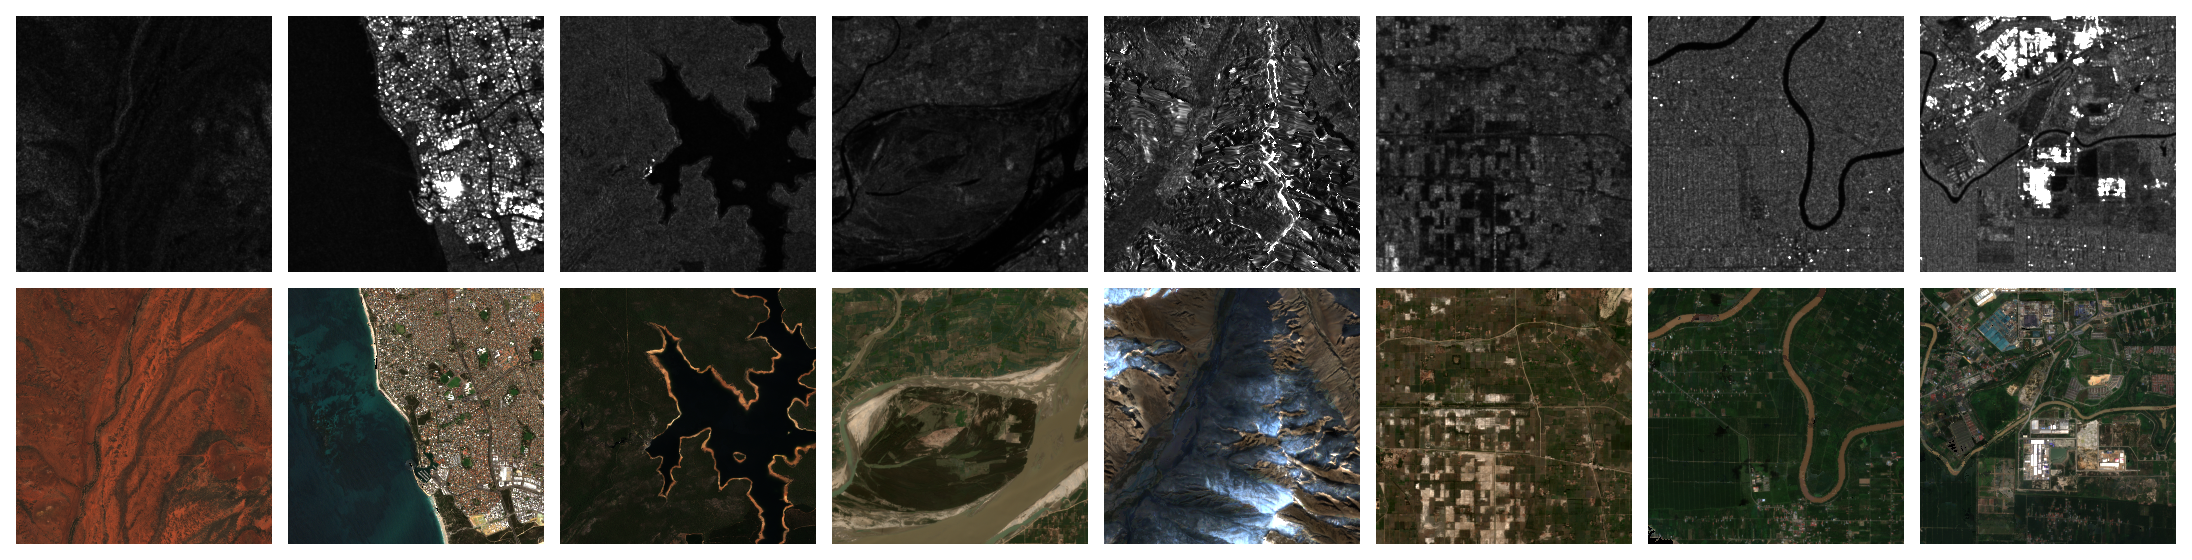
\includegraphics[width=\textwidth]{showCase.png}
    \caption{Sample images from the new added data. Top row: Sentinel-1 images, bottom row: corresponding Sentinel-2 images}
    \label{fig:showCase}
\end{figure*}

\subsection{Dataset availability}
The \textit{Augmented Sentinel 1-2} dataset is shared under the open access license CC-BY-SA 4.0 and is available to download at a persistent link provided by kaggle and DataCite. The dataset can be accessed at \url{https://doi.org/10.34740/kaggle/dsv/11487561}.

All tools used to create the dataset are available at \href{https://github.com/ShambaC/Augmented-SEN-1-2}{GitHub}.

\bibliographystyle{plain}
\bibliography{references}

\end{document}